\section{Disk vertical gravity and lensing around isolated galaxies}
\label{sec:disklensing}

Two galaxy tests measure the gravitating mass away from the rotation
curve. The vertical dispersion of an old disk measures the force
perpendicular to the plane. Weak lensing around isolated galaxies measures
the projected mass out to a few hundred kiloparsecs. On NGC~628 the stock
model and an abundance-matched NFW halo give $\chi^2=2.04$ and 2.01, and
algebraic QUMOND gives 8.86. On the KiDS isolated lenses MOND gives
$\chi^2=110$ with no halo parameter; the stock model gives 171 at the
standard concentration and 132 at three tenths of it, and NFW halos give
252 and 124.

\subsection{Old-disk vertical gravity}
\label{sec:olddisk}

The reduced old-disk solver fits one stellar mass to five old-disk
dispersions of NGC~628 and compares it with the stellar mass required by
the flat rotation speed. A round component adds the vertical term
$(V_h^2/R^2)(\pi^2/3)h_z^2$ to $\langle\sigma_z^2\rangle$ for a
$\mathrm{sech}^2$ layer with $z_0=2h_z$. Algebraic QUMOND multiplies the
disk self-gravity by $\nu(g_N/a_0)$ with the same interpolating function.
\begin{center}
\small
\begin{tabular}{lccc}
\toprule
Model & $\chi^2$ (5 points) & $M_*/10^{10}\Msun$ from $\sigma_z$ & pull against rotation\\
\midrule
Stock completion, $a_0=1.2494$ & 2.04 & 2.60 & $-0.23\sigma$\\
Algebraic QUMOND, $a_0=1.2494$ & 8.86 & 1.01 & $-2.92\sigma$\\
\LCDM, abundance-matched NFW & 2.01 & 2.69 & $-0.69\sigma$\\
\LCDM, halo mass $\pm0.3$~dex & 2.00--2.06 & 2.55--2.82 & $-0.03$ to $-1.28\sigma$\\
Newtonian baryons only & 2.43 & 3.33 & $+0.88\sigma$\\
\bottomrule
\end{tabular}
\end{center}
QUMOND multiplies the vertical self-gravity of the disk and requires a
stellar mass less than half the rotational value. The stock completion and
a round halo add a modest vertical term and agree with the rotation. The
reduced vertical-force test favors the stock model over the specified
algebraic QUMOND approximation and gives the same fit quality as the
round NFW halo. At the exponential fit's normalization
$a_0=1.2588\times10^{-10}\,\mathrm{m\,s^{-2}}$, the corresponding
stock and algebraic QUMOND scores are 2.04 and 8.95, with mass offsets
$-0.21\sigma$ and $-2.91\sigma$. Gas-profile, inclination, and
scale-height uncertainties remain.
\source{U1, S15; X2}

\subsection{Isolated-galaxy lensing}
\label{sec:galaxylensing}
\label{sec:kidsthree}

An isolated finite stock bounds the excess surface density by
$(1+S)g_{\rm bar}/\pi G$. A signal on the deep response law then requires
$S\ge\tfrac\pi4\sqrt{a_0/g_{\rm bar}}-1$: about 12 at
$4.7\times10^{-13}$, 31 at $7.6\times10^{-14}$ and 275 at
$10^{-15}\,\mathrm{m\,s^{-2}}$. Stocks of about 30 fit the inner KiDS
bins \cite{brouwer21}. The carried stock ends with the support,
where hot gas outweighs the condensed baryons, and the uncarried stock
outside keeps the halo profile.

The comparison uses a population forward model of the four isolated
stellar-mass bins of Brouwer et al., with 60 points and the full
covariance. Each model receives the same lens population, the same hot
circumgalactic gas with $f_{\rm hot}=0.2$, the same galaxy point mass,
and the same eight-amplitude environment term. MOND applies the
interpolating function to all baryons, the hot gas included. The NFW
halos and the uncarried stock receive a global halo-mass shift and a
concentration factor (Figure~\ref{fig:kidsthree}).
\begin{center}
\small
\begin{tabular}{lccc}
\toprule
Model & standard $c$ & $c\times0.6$ & best fit\\
\midrule
MOND, no halo parameter & \multicolumn{3}{c}{110.5}\\
Stock model, support-limited & 171.0 & 146.6 & 131.7 ($c\times0.3$)\\
\LCDM, truncated NFW & 252.1 & 154.1 & 124.3 ($c\times0.38$)\\
\bottomrule
\end{tabular}
\end{center}
At the standard and mildly reduced concentrations the stock model fits
better than the NFW halos. Both reach their lowest $\chi^2$ only with
concentrations near a third of the Dutton--Macci\`o relation. There the
NFW minimum, 124.3, lies 7.4 below the lowest stock value on the tested
grid, which sits at the grid edge. MOND fits best of the three, in agreement with Brouwer et
al. and Mistele et al. All models leave $3$--$6\sigma$ residuals at $0.5$--$1.5\,$Mpc, where
neighbouring structure contributes. With the concentration factor held
at 0.6 or above, the profiled NFW minimum is 151.3.
\source{G8, G12; X3}\cite{brouwer21,kidsnew}

\begin{figure}[htbp]
\centering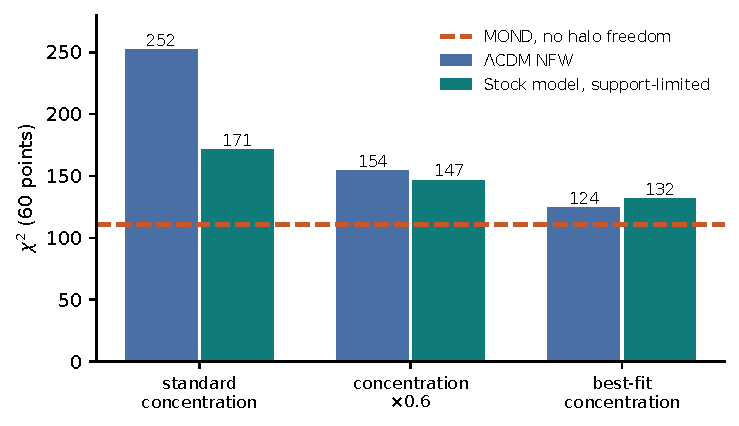
\includegraphics[width=0.75\textwidth]{figures/kids_three.pdf}
\caption{KiDS isolated-lens $\chi^2$ over 60 points with the full
covariance. NFW halos and the uncarried stock are shown at the standard
concentration, at 0.6 of it, and at their best-fit concentration factor
(0.38 for NFW and the grid edge 0.3 for the stock). The values at
standard and $0.6\times$ concentration are minima over the same grid of
halo-mass shifts for both models. The dashed line is
MOND with all baryons, the hot gas included, as source.}
\label{fig:kidsthree}
\end{figure}

The published acceleration table of Mistele et al. gives a diagonal statistic of
10.06 for fifteen bins at the reference $a_0$, or 5.99 for seven inner
bins, including the tabulated statistical and interpolation/extrapolation
uncertainties. Its full covariance was unavailable and its published $H_0=73$
convention was retained. This reduction overlaps the profile data and
adds no independent evidence. \source{U1, S04}

